\documentclass[../user-manual.tex]{subfiles}
\begin{document}
	
	В данной главе рассматриваются вопросы формирования и выгрузки отчётов. Все примеры построены на основе объектов, создаваемых в качестве учебных примеров в главе \ref{chapter:developing}.
	
	\section{Запуск отчёта}
	
	Пользователю, обладающему правами на выполнение отчётов (система прав Магрепорт описана в главе \ref{chapter:administration}) доступны следующие пункты бокового меню:
	\begin{itemize}
		\item \textbf{Отчёты} --- в этом пункте меню пользователь может осуществлять навигацию по каталогам с отчётами и запускать отчёты на выполнение.
		
		\item \textbf{Избранное} --- в этом пункте меню пользователь видит отчёты, отмеченные им как избранные и может запускать их на выполнение.
		
		\item \textbf{Задания} --- в этом пункте меню пользователь видит свои выполненные задания, может просматривать их результат, а также перезапускать отчёт на новое выполнение с фильтрами, заполненными как в данном задании.
	\end{itemize}


	\begin{NB}
		\textit{Отчётом} в системе Магрепорт называется объект, позволяющий пользователю осуществлять выгрузку данных из БД. Чтобы не возникало терминологической путанницы, сформированный при помощи этого объекта отчёт с конретными выгруженными из БД данными в Магрепорте называется \textit{заданием}. Сами полученные данные назваются при этом \textit{выгруженными данными} или \textit{данными задания}.
	\end{NB}
	
	
	\begin{figure}[h]
		\centering
		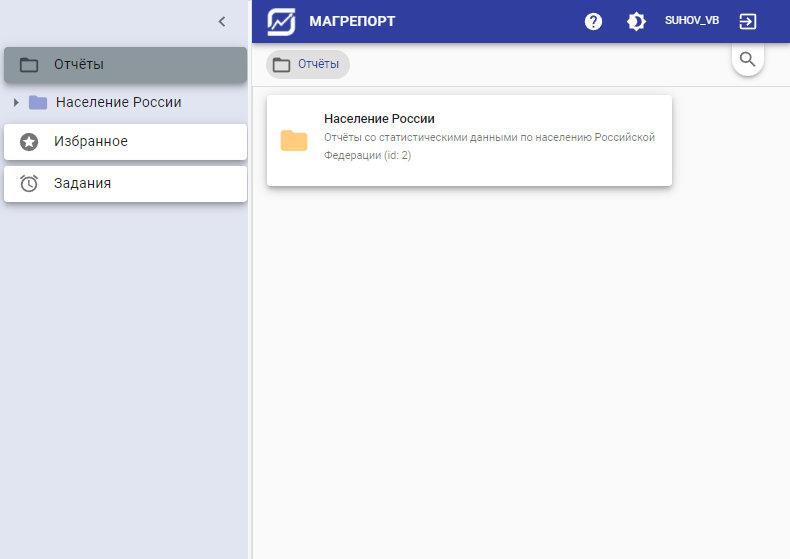
\includegraphics[width=\graphicswidth]{img/1-folders.png}
		\caption{Навигация по каталогам}
		\label{fig:folders}
	\end{figure}
	
	При клике на карточку отчёта (см. рис. \ref{fig:report-card}) в разделах <<Отчёты>> и <<Избранное>> или на кнопку перезапуска задания на карточке задания в разделе <<Задания>> (см. рис. \ref{fig:restart-task-button}) пользователь переходит в мастер запуска отчёта, позволяющий задать значения фильтров отчёта (см. рис. \ref{fig:set-report-filters}). Если в отчёте нет фильтров, в результате этого действия отчёт сразу будет запущен на выполнение. В мастере задания значений фильтров фильтры будут иметь те значения, которые были заданы при последнем запуске пользователем этого отчёта (в случае запуска отчёта через клик на карточке отчёта) либо при запуске перезапускаемого задания (в случае клика на кнопку <<Запустить отчёт заново>>). При первом запуске отчёта пользователем, а также если в отчёт были внесены какие-либо изменения, фильтры отображаются незаполненными. Все фильтры можно очистить (удалить выбранные значения) нажатием кнопки <<Очистить>>. После задания значений фильтров пользователь может запустить отчёт на выполнение, нажав кнопку <<Выполнить>>.
	
	\begin{figure}[h]
		\centering
		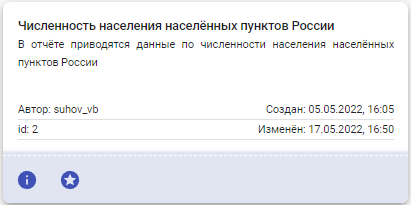
\includegraphics[width=\graphicswidth]{img/2-report-card.png}
		\caption{Карточка отчёта}
		\label{fig:report-card}
	\end{figure}	
	
	\begin{figure}[h]
		\centering
		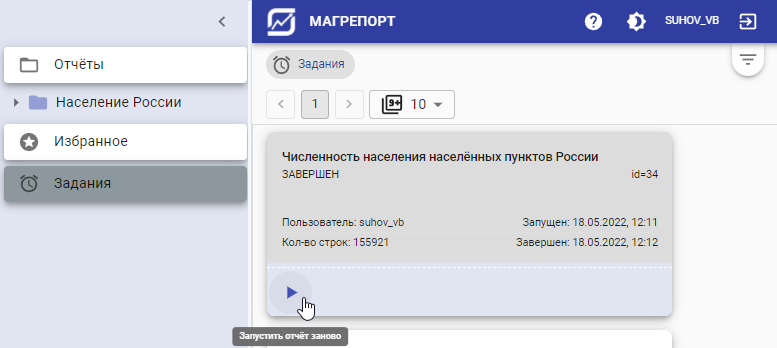
\includegraphics[width=\graphicswidth]{img/3-restart-task-button.png}
		\caption{Кнопка перезапуска задания}
		\label{fig:restart-task-button}
	\end{figure}

	\begin{figure}[h]
		\centering
		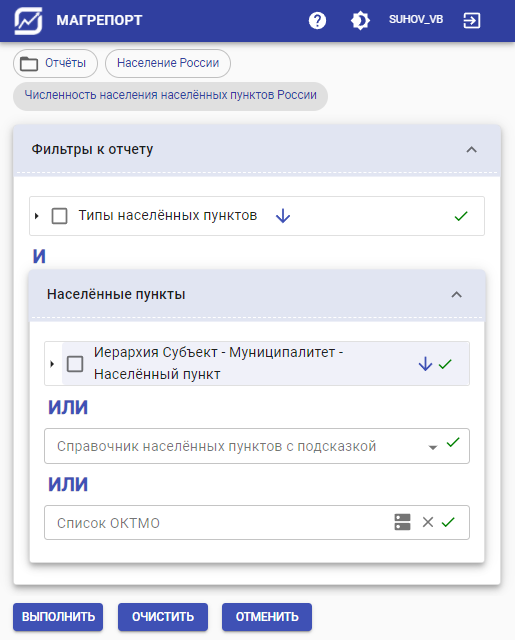
\includegraphics[width=\graphicswidth]{img/4-set-report-filters.png}
		\caption{Мастер задания значений фильтров отчёта при запуске}
		\label{fig:set-report-filters}
	\end{figure}

	После запуска отчёта создаётся новое задание. Пользователь при этом попадает в мастер просмотра задания. Если выполнение задания ещё не завершено, в мастере просмотра задания пользователю отображается крутящийся спиннер и кнопка <<Отменить>>, при нажатии на которую пользователь может отменить выполнение задания. Пользователю не обязательно оставаться в мастере просмотра задания до момента завершения его выполнения --- задание выполняется независимо от того, ожидает ли пользователь завершения выполнения задания в мастере просмотра задания или продолжает работу с приложением, в том числе запускает другое задание.
	
	Список заданий пользователя отображется в разделе <<Задания>> в виде карточек заданий (см. рис. \ref{fig:restart-task-button}). На карточке задания отображен статус выполнения задания. Обновить список заданий можно нажав кнопку <<Обновить>> в правом нижнем углу окна. Статусы выполнения заданий:
	
	\begin{itemize}
		\item \textbf{В ОЧЕРЕДИ} --- задание ожидает старта выполнения в очереди в Магрепорт
		
		\item \textbf{ВЫПОЛНЯЕТСЯ} --- задание выполняется на БД
		
		\item \textbf{ЭКСПОРТ} --- задание выполнено на БД, производится экспорт в файл Excel по умолчанию.
		
		\item \textbf{ЗАВЕРШЕН} --- задание выполнено, файл Excel экспортирован.
		
		\item \textbf{ЗАВЕРШЕН С ОШИБКОЙ} --- задание завершено с ошибкой.
		
		\item \textbf{ОТМЕНЯЕТСЯ} --- запущена отмена задания, производится отмена выполнения запроса на стороне БД.
		
		\item \textbf{ОТМЕНЕН} --- задание отменено пользователем или администратором.
		
	\end{itemize}

	\begin{devnote}
		Для каждого источника данных (см. главу \ref{chapter:developing}) задаётся размер пула коннектов. При полной утилизации пула задания попадают в очередь в Магрепорте и ожидают освобождения ранее занятых коннектов, в этом случае они находятся в статусе \textit{В ОЧЕРЕДИ}.
	\end{devnote}

	Дождавшись завершения выполнения запущенного отчёта из мастера запуска отчётов или кликнув на карточке задания со статусом \textit{ЗАВЕРШЕН} или \textit{ЗАВЕРШЕН С ОШИБКОЙ}, пользователь оказывается в выполненном задании. Если задение завершено с ошибкой, пользователь видит информационное сообщение с текстом ошибки, если задание завершено успешно --- пользователь оказывается в мастере работы с выполненным отчётом.
	
	\section{Работа с выполненным отчётом}
	
	В мастере работы с выполненным отчётом отображаются данные выполненного отчёта в табличной форме (см. рис. \ref{fig:report-data}).
		
	\begin{figure}[h]
		\centering
		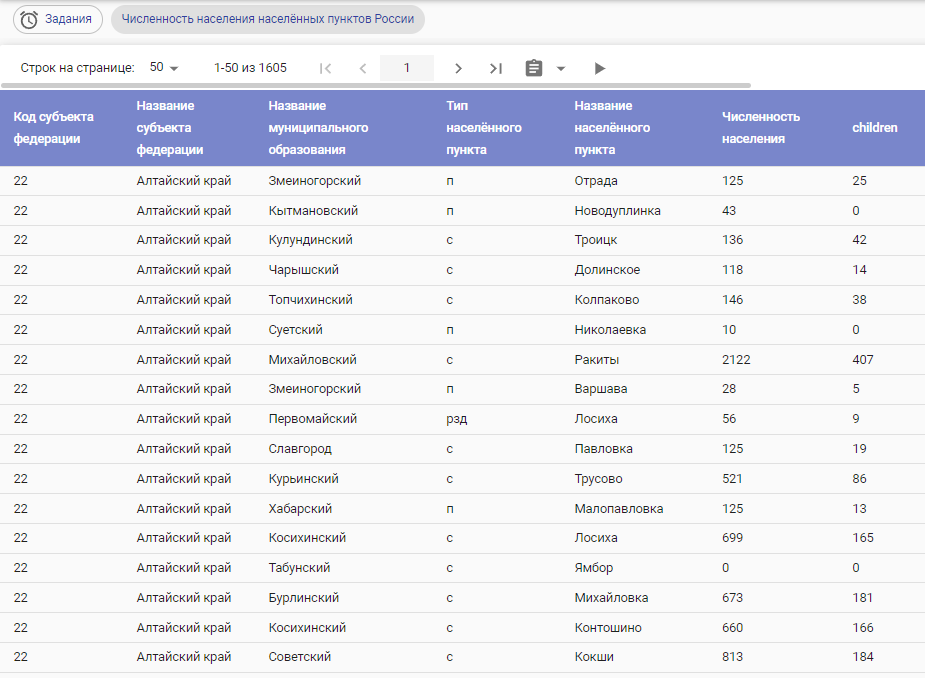
\includegraphics[width=\graphicswidth]{img/6-report-data.png}
		\caption{Данные выполненного отчёта}
		\label{fig:report-data}
	\end{figure}	

	Одномоментно на странице отображается некоторое количество строк, управляемое параметром <<Строк на странице>> (по умолчанию 50). При помощи кнопок навигации по страницам можно перелистывать страницы, общее количество строк в отчёте и просматриваемый диапазон строк на текущей странице показан в верхней строке рядом с кнопками навигации.
	
	Следом за кнопками навигации по страницам идёт кнопка выгрузки результатов отчёта в Excel (<<Экспорт Excel>>). При нажатии на кнопку отчёт выгружается с использованием шабллона по умолчанию. Рядом расположена кнопка выбора шаблона выгрузки (<<Дополнительные шаблоны экспорта>>), следом идёт кнопка перезапуска отчёта. При перезапуске отчёта происходит переход в мастер задания значений фильтров, при этом в фильтры подставляются те значения, которые были указаны при выполнении отчёта.
	
	\section{Раздел <<Задания>>}
	
	В разделе <<Задания>> приводятся карточки выполненных пользователем заданий и выполненных по расписанию для пользователя заданий. Задания, выполненные по расписанию, выполняются от имени поьлзователя \textit{MAG\_SCHEDULE\_USER}. В правом нижнем углу окна находится кнопка <<Обновить>>. По нажатию кнопки обновляется список заданий и их статусы.
	
	\section{Раздел <<Избранное>>}
	
	Пользователь может добавить отчёт в персональный раздел <<Избранное>> --- соответствующая кнопка расположена на карточке отчёта (см. рис. \ref{fig:add-to-favorites}). Повторный клик на данной кнопке удаляет отчёт из списка избранных. Список избранных отчётов находится в разделе <<Избранное>>.
	
	\begin{figure}[h]
		\centering
		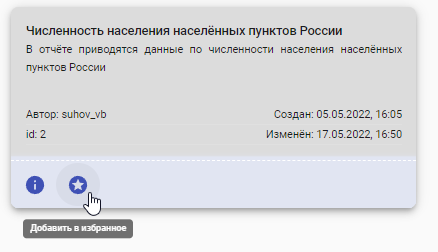
\includegraphics[width=\graphicswidth]{img/5-add-to-favorites.png}
		\caption{Кнопка добавления отчёта в избранное}
		\label{fig:add-to-favorites}
	\end{figure}	
	
\end{document}